
\section{Semantic Segmentation} \label{sec:3.1}
A large field of models in Deep Learning are discriminative models. A simple version of a discriminative model would be a classifier. A classifier given an input $\vec{x}$ outputs a scalar class value $y\in\vec{y}$ of the input where $\vec{y}$ is a set of classes (which are also called labels). The simplest classifier would be a binary classifier that places an input into one of two classes, e.g. deciding if an image shows a cat or a dog. More advanced classifiers identify way more classes. A classical example would be a classifier trained on the CIFAR-10 dataset \cite{cifar10}, which contains millions of $32\times32$ pixel images categorized by $10$ classes (car, airplane, dog, $\dots$).

The above described classifiers always assign one scalar value to an input. Semantic Segmentation Networks also assign scalar values, but not one value per image, but one value per pixel! This already reveals a lot about the application of such networks. They operate on images and their task is to assign each pixel in the image a class. For example, given the image of a street scene a semantic segmentation network tries to classify each individual pixel as part of a car, a street, a building, $\dots$\,.
%
\begin{figure} \label{fig:3.1}
    \centering
    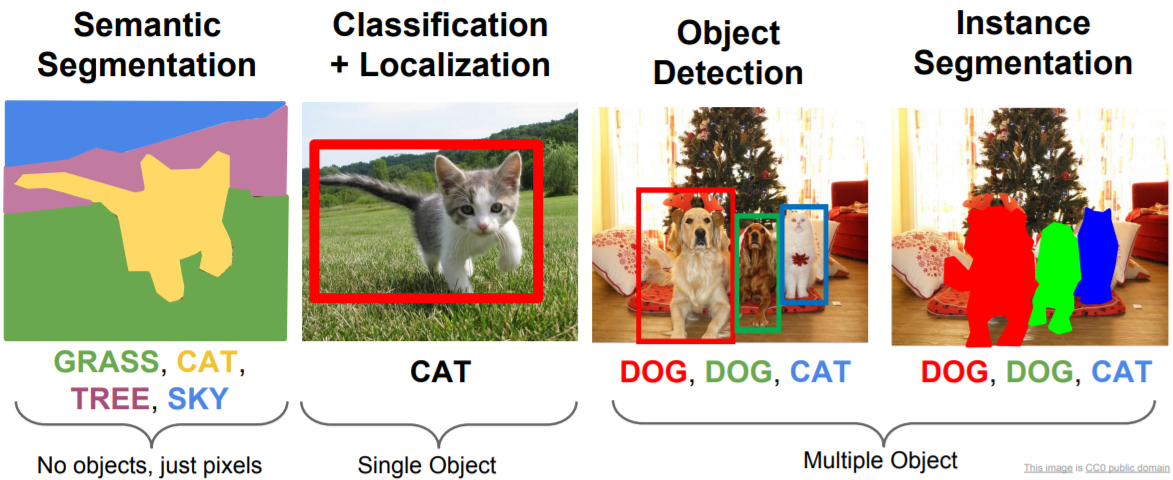
\includegraphics[width=.8\textwidth]{Chapters/figures/sem_seg.PNG}
    \caption[Overview of various computer vision tasks]{Overview of various computer vision tasks. Figure from\\ http://cs231n.stanford.edu/slides/2017/cs231n\_2017\_lecture11.pdf.}
\end{figure}
%

There are also modifications of semantic segmentation for example instance segmentation. In instance segmentation, not only is each pixel assigned a class, but also the different instances of objects in an image are specified. An overview of semantic segmentation and related techniques is shown in \hyperref[fig:3.1]{Fig.\,3.1}

As we will see in \hyperref[sec:4.5]{Sec.\,4.5} and \hyperref[chap:5]{Chapter 5}, semantic segmentation networks are necessary to make semantic image synthesis possible with Score-Based Generative Models. Therefore, the semantic segmentation models used in later work are briefly explained below:
%
\subsection{FCN} \label{sec:3.1.1}
FCN \cite{fcn} stands for \textit{Fully Convolutional Network} and is a semantic segmentation network whose architecture is inspired by successful image classification networks such as VGGNet \cite{vgg}. 

VGGNet in principle works by first downsampling an image with several convolution layers, followed by a few fully connected layers. The last fully connected layer then gives the probabilities of the image being of a certain class. An overview of this architecture is presented in \hyperref[fig:3.2]{Fig.\,3.2}.
%
\begin{figure} \label{fig:3.2}
    \centering
    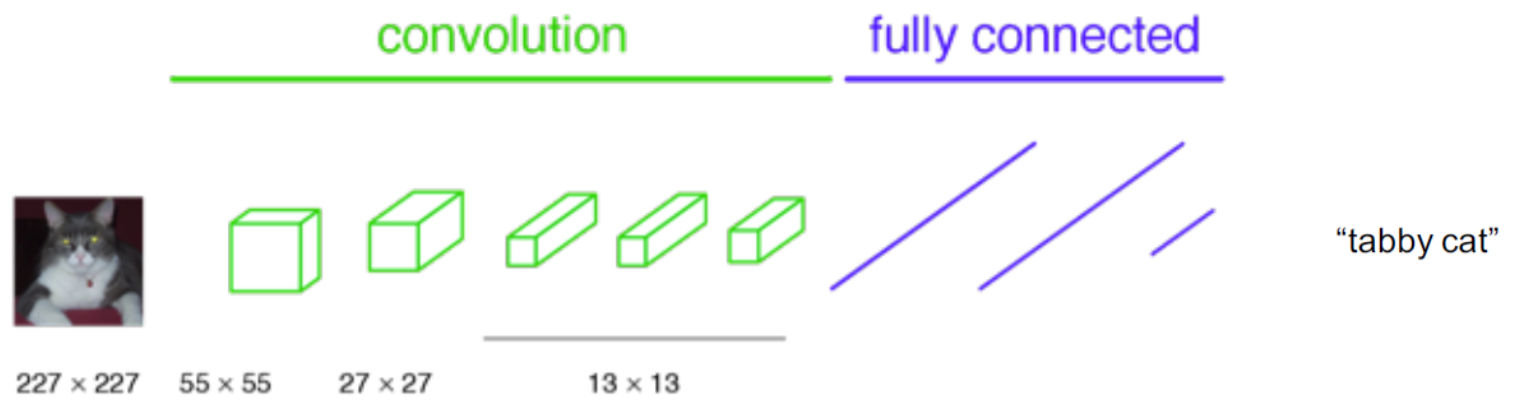
\includegraphics[width=.65\textwidth]{Chapters/figures/vgg.PNG}
    \caption[The architecture of classification networks]{The architecture of classification networks such as VGGNet. Figure from\\ https://towardsdatascience.com/review-fcn-semantic-segmentation-eb8c9b50d2d1.}
\end{figure}
%
%
\begin{figure}[b] \label{fig:3.3}
    \centering
    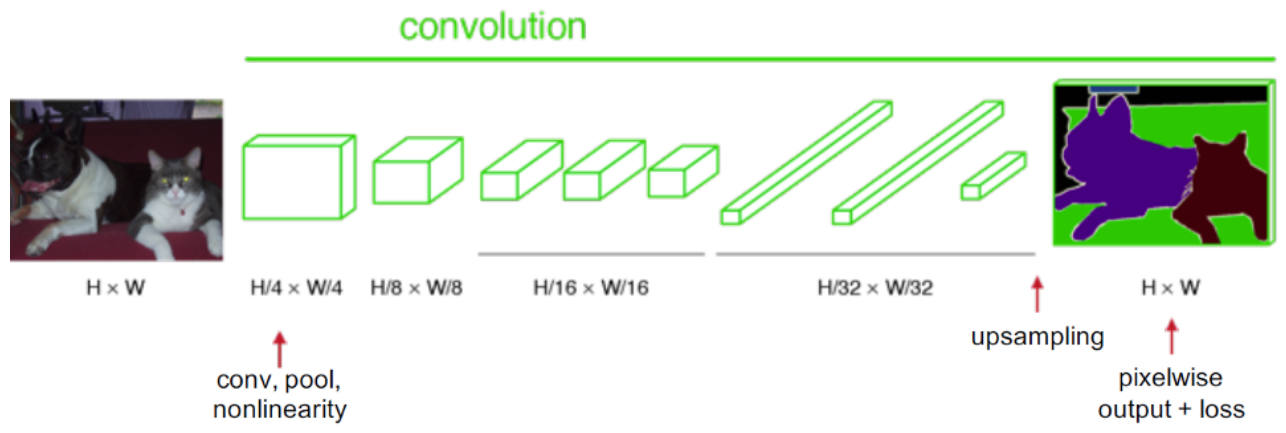
\includegraphics[width=.65\textwidth]{Chapters/figures/fcn.PNG}
    \caption[The FCN architecture]{The FCN architecture. Figure from \cite{fcn}.}
\end{figure}
%

FCN builds on this architecture by replacing the fully connected layers with $1\times1$ convolution layers. The entire architecture – seen in \hyperref[fig:3.3]{Fig.\,3.3} – then consists of successive blocks operating on different fractions of the original resolution. Each block consists of a convolution layer, a max pooling layer and an activation function. To move from the pixel-wise $H/32\times W/32$ prediction to a prediction of the original resolution, an upsampling process (\hyperref[fig:3.4]{Fig.\,3.4}) is deployed. The problem with this is that the lower resolutions are needed to capture fine details in the original picture but the spatial location of this features is almost completely lost. Therefore, the outputs after the pooling layers for \textit{each} resolution are consecutively combined during the upsampling procedure to get back the spatial information. These cross connections between the downsampling and the upsampling part of the network are called \textit{skip connections}.

%
\begin{figure} \label{fig:3.4}
    \centering
    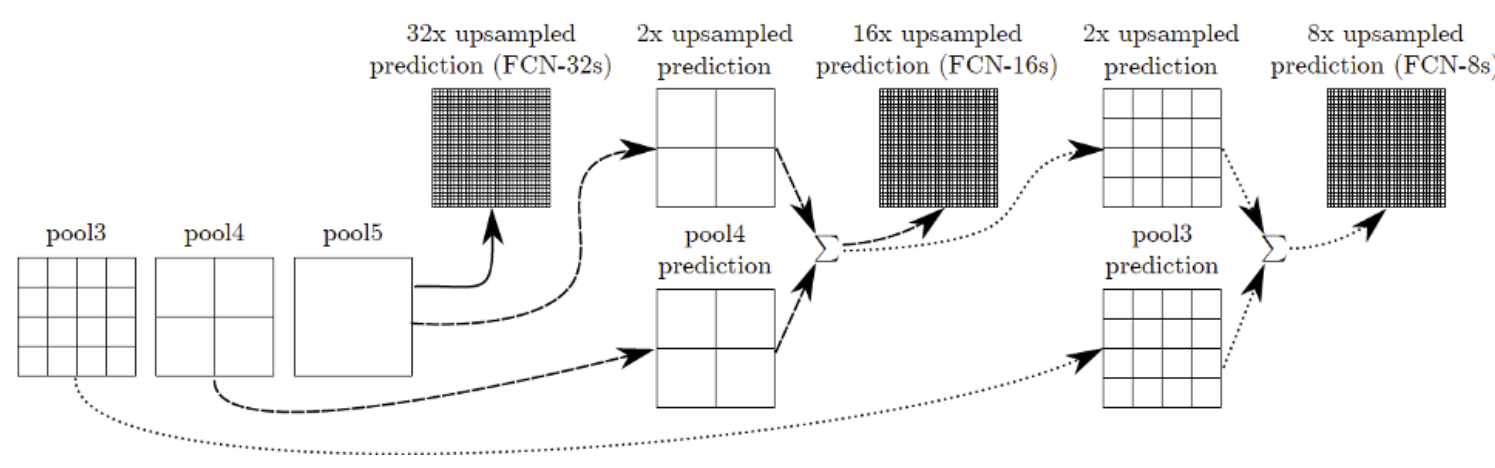
\includegraphics[width=.65\textwidth]{Chapters/figures/fcn2.PNG}
    \caption[FCN upsampling process]{Upsampling by successively combining the output of all max pooling layers. Image from \cite{fcn}}
\end{figure}
%
\subsection{U-Net} \label{sec:3.1.2}
U-Net \cite{unet} is an adaption of the fully convolutional structure of FCNs (\hyperref[sec:3.1.1]{Sec.\,3.1.1}) and initially was designed for applications in biomedical image segmentation. Looking at the network architecture in \hyperref[fig:3.5]{Fig.\,3.5} it quickly becomes clear where the name U-Net originates from.
%
\begin{figure}[h!] \label{fig:3.5}
    \centering
    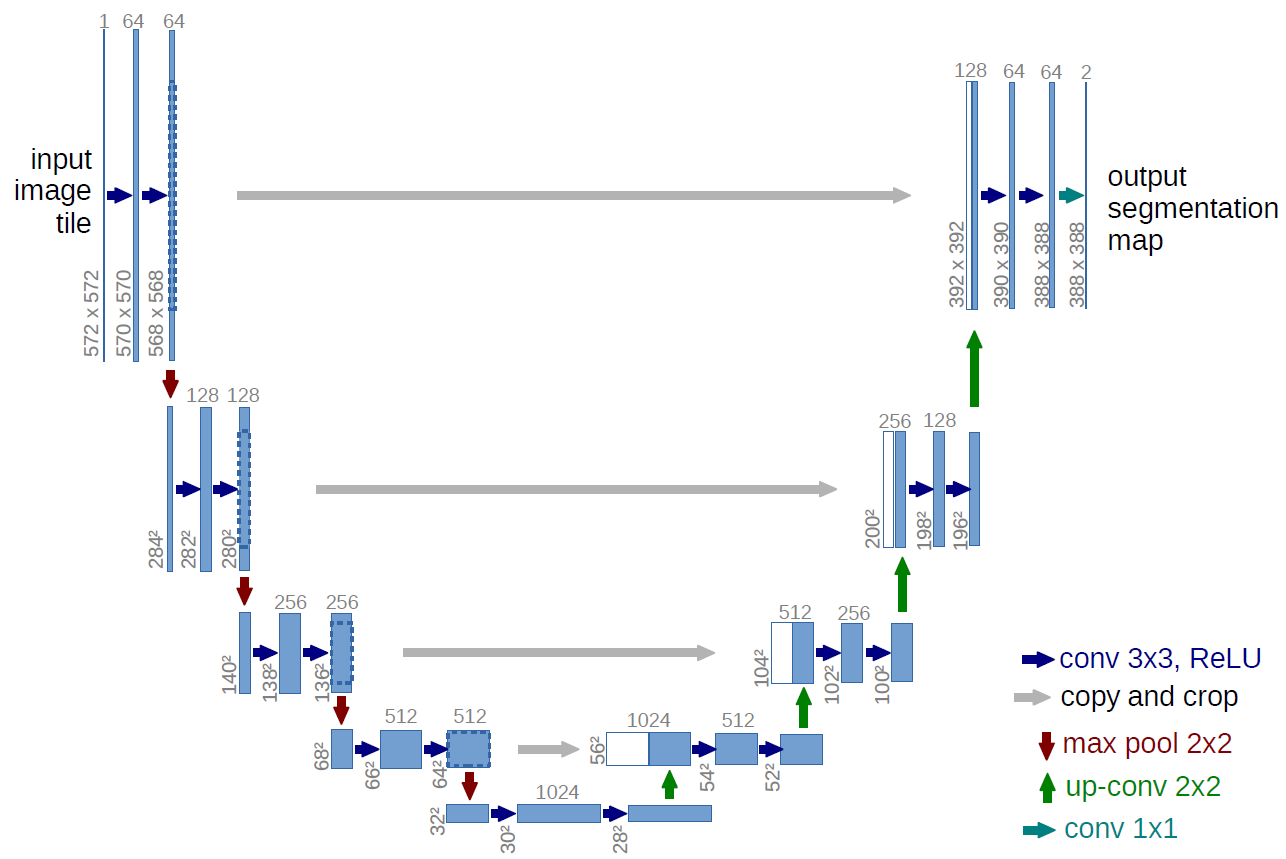
\includegraphics[width=.70\textwidth]{Chapters/figures/unet.PNG}
    \caption[The U-Net architecture]{The U-Net architecture. Figure from \cite{unet}.}
\end{figure}
%

As with FCNs the U-Net architecture consists of a downsampling part and an upsampling part which are connected by skip connections. The main modification in U-Net is that the upsampling part has a lot more feature channels than in FCNs which allows the network to better propagate feature information to higher resolution. In general, the U-Net achieved better results than FCN and needs a lot less training samples to achieve good predictions \cite{unet}.

%%%%%%%%%%%%%%%%%%%%%%%%%%%%%%%%%%%%%%%%%%%%%%%%%%%%%%%%%%%%%%%%%%%%%%%%%%%%%%%%%%%%%%%%%%%%
\section[Generative Modeling – VAEs and GANs]{Generative Modeling – VAEs and GANs%
    \sectionmark{Generative Modeling}}
\sectionmark{Generative Modeling}
There are mainly two types of models: \textit{Generative Models} and \textit{Discriminative Models}. The latter discriminate between different kind of data instances, e.g. discriminate images of cats and dogs. Semantic Segmentation Models (\hyperref[sec:3.1]{Sec.\,3.1}) are discriminative models. Given a data instance $\vec{x}$ and a set of labels $\vec{y}$ discriminative models learn the conditional probability $p(\vec{y}|\vec{x})$. Generative models generate new data instances. They capture the joint probability $p(\vec{x},\vec{y})$ or $p(\vec{x})$ if there are no labels. In general, generative models are a lot harder than discriminate models. There are various approaches to generative modeling, the most popular being Variational Autoencoders (VAEs) \cite{vae_original} and Generative Adversarial Networks (GANs) \cite{gan_original}:

\subsubsection{Variational Autoencoders}
Although VAEs \cite{vae_original} do not play a major role in this thesis, they are briefly discussed due to their strong influence in modern generative modeling. In order to understand VAEs one must first understand what an autoencoder is. Autoencoders tackle the problem of encoding and decoding data with minimum information loss. Data generally is described by some abstract features which often form a high dimensional space. The task of an autoencoder is to learn to reduce the dimensionality of this high dimensional features by selecting important old features (selection) or creating less, new features based on the old features (extraction). The arising feature space is called \textit{latent space} which essentially only contains the most important features of the input data. To learn such an encoding the autoencoder network consists of an encoder network $E(\vec{x})$ and a decoder network $D(\vec{x})$. An input $\vec{x}$ is first encoded by the encoder to a low dimensional value $\vec{z}$ which then is decoded by the decoder to an output $\tilde{\vec{x}}$ of the same dimension as the input. Thereafter the input $\vec{x}$ is compared to the output $\tilde{\vec{x}}$ and the network gets punished for differences between input and output.

An autoencoder thus learns to compress and decompress data in the best possible way without loss of information. A na\"{i}ve way to now generate new data via a trained autoencoder is to use the decoder to decode a random sample from the latent space. The problem with this approach is that the autoencoder learns to best possible compress the data. As a consequence, we cannot sample from the latent space because the distribution in latent space has no meaning w.r.t the real data. For example, if you decode the image of a car into the latent space and then change the latent representation of the car just a little, after decoding you will most likely see noise instead of an image of a new car. In mathematical terms this means that the latent space of an autoencoder is not regularized.

A VAE solves this problem by ensuring that the latent space has good properties that enable generative modeling while still learning to encode the data in an efficient way. In order to do so the encoder of a VAE does not encode an input $\vec{x}$ to a single value but to a distribution in latent space $p(\vec{z}|\vec{x})$. The decoder then decodes a sample $\vec{z}\sim p(\vec{z}|\vec{x})$ to an output $\tilde{\vec{x}}$ which is compared to the output to compute a reconstruction loss. Furthermore, a regularization loss is computed assuring that $p(\vec{z}|\vec{x})\sim\mathcal{N}(\vec{0},\vec{I})$. The regularized latent space has the very useful property that similar data is close together. So now, if the decoder is given a slightly different latent representation of a car, it would decode it into a new image of a car. An overview of the VAE network architecture can be seen in \hyperref[fig:3.6]{Fig.\,3.6}
%
\begin{figure} \label{fig:3.6}
    \centering
    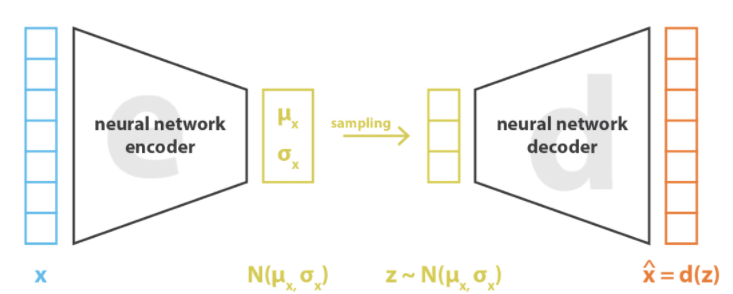
\includegraphics[width=.65\textwidth]{Chapters/figures/vae.PNG}
    \caption[Basic VAE model architecture]{Basic VAE model architecture. Figure from\\
    https://towardsdatascience.com/understanding-variational-autoencoders-vaes-f70510919f73}
\end{figure}
%
\subsubsection{Generative Adversarial Networks} \label{sec:gans}
GANs were proposed in 2014 \cite{gan_original} and have since seen great success and a lot of adaptions. GANs work by combining two models: A generator model and a discriminator model. These two models are trained at the same time and have an adversarial relationship to each other. Adversarial in that sense means that the generator and discriminator have opposing objectives. 

The generator $G(\vec{x})$ has the task of generating samples of the data distribution $p_{data}(\vec{x})$. The discriminator $D(\vec{x})$ has the role of distinguishing the generated data $\tilde{\vec{x}}$ from the real data $\vec{x}$. To be more precise, the task of the generator is to best possible trick the discriminator that at the same time has the task to best possible decide if an image is real or fake (generated). If the discriminator correctly identifies a generated image as fake the generator is punished to produce better images. Obviously, "better" just means that the images are more likely to fool the discriminator, which does not necessarily equate to a real-looking image if the discriminator performs poorly. When the discriminator is deceived by the generator, it is punished to better discriminate real and fake images. While GANs can produce excellent samples and are fast at sampling, it is easy to imagine how hard it is to train two networks at the same time. If not properly adjusted training quickly becomes unstable.

The absolute error of the discriminator can be written in the following way:
%
\begin{equation}
    E(G,D)=\frac{1}{2}\left(\mathbb{E}_{\vec{x}\sim p_{t}}[1-D(\vec{x})]+\mathbb{E}_{\vec{x}\sim p_{z}}[D(G(\vec{z}))]\right)
\end{equation}
%
Here $\vec{x}$ is an input to the discriminator and $\vec{z}$ is a random input to the generator. Rewriting $G(\vec{z})$ as an input to the discriminator yields
%
\begin{equation} \label{equ:3.2}
    E(G,D)=\frac{1}{2}\left(\mathbb{E}_{\vec{x}\sim p_{t}}[1-D(\vec{x})]+\mathbb{E}_{\vec{x}\sim p_{g}}[D(\vec{x})]\right),
\end{equation}
%
where $\vec{x}$ can either be a real input ($\vec{x}\sim p_t$) or a generated input ($\vec{x}\sim p_g$). Therefore, in \hyperref[equ:3.2]{Equ.\,3.2} the left term describes the error of falsely classifying a real image as generated and the right term describes the error of falsely classifying a generated image as real. From this it can be deduced that the perfect discriminator $D^*(\vec{x})$ classifies a real image as $1$ and a fake image as $0$. 

The total model objective of GANs can be written as 
%
\begin{equation} \label{equ:3.3}
    \underset{G}{\max}\left(\underset{D}{\min}\,E(G,D)\right),
\end{equation}
%
which can be interpreted as the discriminator trying to minimize its error, while at the same time the generator tries to maximize the discriminator's error. A sketch of the training procedure is shown in \hyperref[fig:3.7]{Fig.\,3.7}. 
%
\begin{figure} \label{fig:3.7}
    \centering
    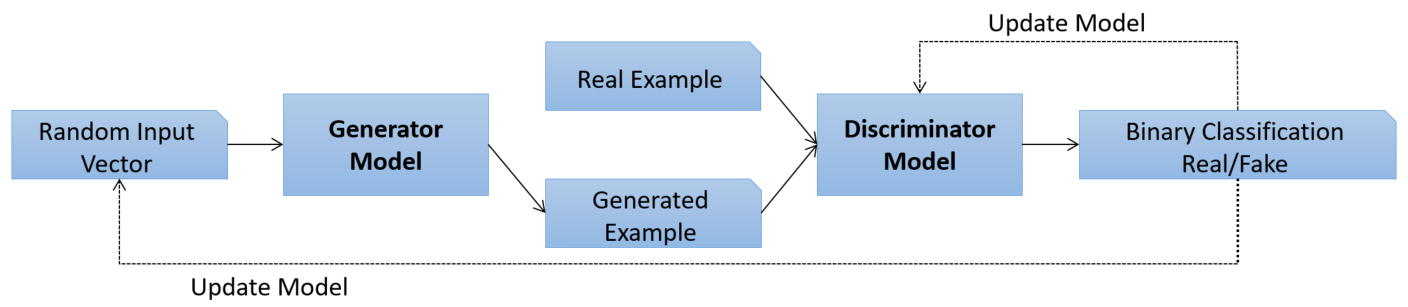
\includegraphics[width=.9\textwidth]{Chapters/figures/gan.PNG}
    \caption[Basic GAN model architecture]{Basic GAN model architecture}
\end{figure}
%

In this thesis the results of our score-based generative semantic image synthesis model are compared with the results of state-of-the-art models of different architecture. All models used for comparison are briefly explained below:

\subsection{Cascaded Refinement Networks} \label{sec:3.2.1}
Photographic Image Synthesis with Cascaded Refinement Networks (CRN) \cite{crn}, a work from 2017, proposed one of the first models being able to synthesize convincing photographic
%
\begin{wrapfigure}{r}{0.45\textwidth}
    \begin{center}
        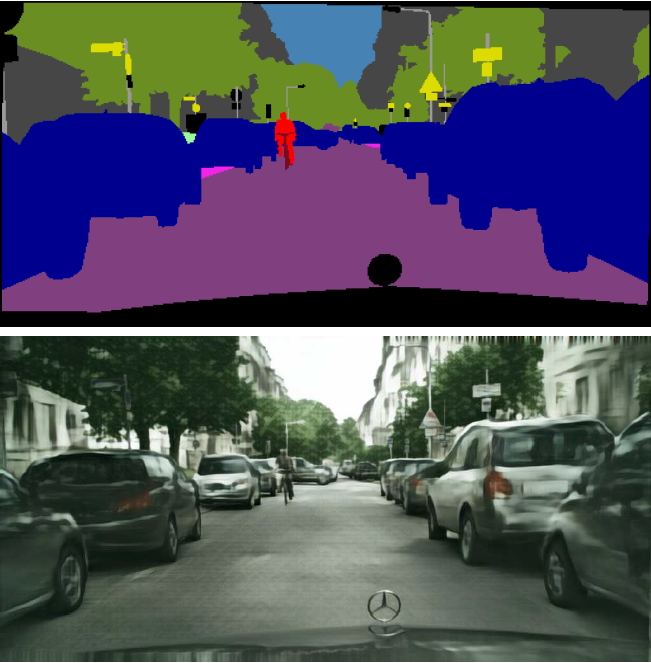
\includegraphics[width=0.43\textwidth]{Chapters/figures/crn_example.PNG}
    \end{center}
    \caption[]{\textit{Top}: Semantic map, \\\textit{Bottom}: Sample image}
\end{wrapfigure}
%
looking images from semantic maps. Unlike other popular models to that time the proposed model does not depend on adversarial training, therefore is no GAN. In fact, CRN is a simple feedforward convolutional network, so it is not a VAE either. Actually, due to the fact that the generated image is fixed for each input (i.e. non-probabilistic), CRN is not even considered a true generative model. The reason to try a feedforward model for image generation is mainly due to the problems of other models (mostly GANs) at that time. There especially were problems of GANs not scaling up to higher resolution \cite{crn}. Also, GANs back then were very unstable to train and therefore "remain remarkably difficult to train"
\cite{crn}.

The CRN works as a cascade of refinement modules $M^i$. Each refinement module consists of three layers: The input layer, an intermediate layer and the output layer. Each of these layers is followed by a $3\times3$ convolution, a layer normalization and a LReLu activation function. 

The input to a refinement module $M^i$ is of size $w_i\times h_i\times(c + d_{i-1})$. Here $w_i\times h_i\times c$ is a downsampled version of the target segmentation map. Normally $w_0\times h_0=4\times 8$ and the downsampling resolution doubles for every module, i.e. $w_i\times h_i=2w_{i-1}\times2h_{i-1}$. $c$ is the channel dimension of the semantic map in one-hot encoding and $d_{i-1}=d_{i-2}+c$. The outputs of a refinement module therefore are convolutional feature layers $F_i$ of size $w_i\times h_i$ which contain $d_i=d_{i-1}+c$ feature maps. In order for this output of size $w_i\times h_i\times d_i$ to be concatenated into the input of layer $M^{i+1}$, which expects an input of size $w_{i+1}\times h_{i+1}\times (c + d_i)$, the output feature maps are up-sampled to resolution $w_{i+1}\times h_{i+1}$.

To the final output feature maps $F^{\bar{i}}$ of module $M^{\bar{i}}$ a $1\times1$ convolution (linear projection) is applied to get from the output of size $w_{\bar{i}}\times h_{\bar{i}}\times d_{\bar{i}}$ to a color image of size $w_{\bar{i}}\times h_{\bar{i}}\times3$.

\subsection{pix2pixHD} \label{sec:3.2.2}
%
\begin{wrapfigure}{r}{0.45\textwidth}
    \begin{center}
        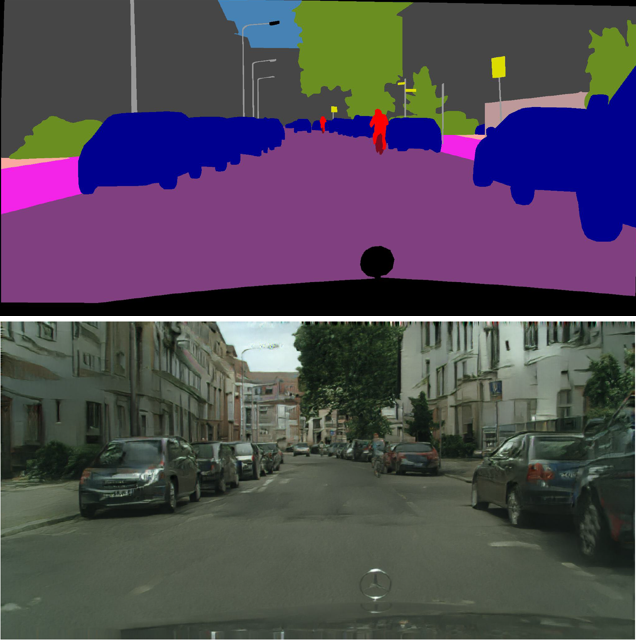
\includegraphics[width=0.43\textwidth]{Chapters/figures/pix2pixHD_example.PNG}
    \end{center}
    \caption[]{\textit{Top}: Semantic map, \\\textit{Bottom}: Sample image}
\end{wrapfigure}
%
pix2pixHD \cite{pix2pixHD} is the successor of the older pix2pix \cite{pix2pix} framework and was developed by scientists of NVIDIA Corporation. pix2pixHD is a GAN model which is able to produce realistic high resolution semantic synthesized images and therefore mitigates the two main concerns of previous GAN models: resolution and image quality. In their paper the authors of pix2pixHD show that their model is able to produce samples of higher quality and realism than CRN (\hyperref[sec:3.2.1]{Sec.\,3.2.1}).

The pix2pix framework works as a classical conditional GAN model in a supervised setting. The generator $G$ has the task to translate a given semantic map to a realistic-looking image, while the discriminator $D$ has the task to distinguish between generated image and the original image for the semantic map.

The pix2pixHD model improves this framework by proposing a coarse-to-fine generator and a multi-scale discriminator. The coarse-to-fine generator essentially is a generator made up of multiple single generators ${G_1, G_2, \dots}$ gradually working on higher resolutions of the image. The multi-scale discriminator addresses the need for a high receptive field for high resolution discrimination. Normally to achieve a higher receptive field either a deeper network or larger convolutional kernels are needed, both leading to increased model capacity and potentially overfitting. Therefore, the multi-scale discriminator consists of three individual discriminators $D_1, D_2, D_3$ each operating on different resolutions. In accordance with the GAN objective in \hyperref[equ:3.3]{Equ.\,3.3} becomes
%
\begin{equation}
    \underset{G}{\min}\underset{D_1,D_2,D_3}{\max}\sum_{k=1,2,3}E(G,D_k)\,.
\end{equation}
%
The generator $G$ is not indexed because the generators $G_i$ are not trained concurrently but one after the other.

\subsection{SPADE} 
%
\begin{wrapfigure}{r}{0.45\textwidth}
    \begin{center}
        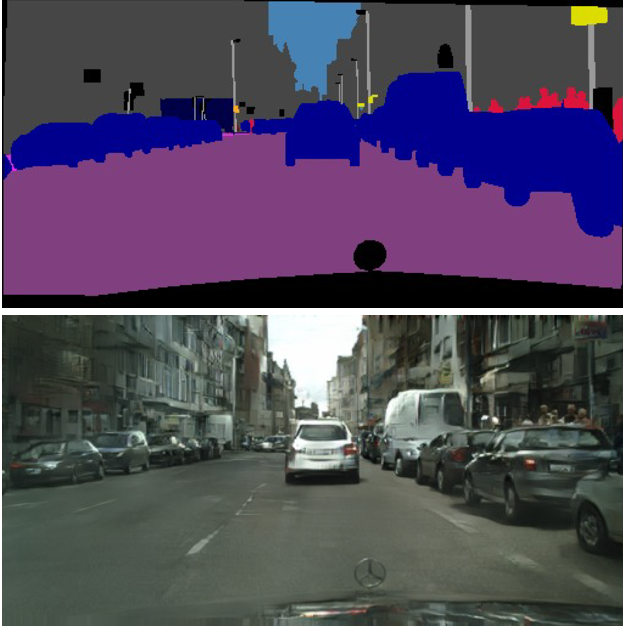
\includegraphics[width=0.43\textwidth]{Chapters/figures/spade_example.PNG}
    \end{center}
    \caption[]{\textit{Top}: Semantic map, \\\textit{Bottom}: Sample image}
\end{wrapfigure}
%
SPADE \cite{spade} actually is no model itself, but the proposal of a new layer for semantic image synthesis: The \textbf{SP}atially-\textbf{A}daptive (\textbf{DE}-)Normalization Layer. In their paper the authors test their new layer as an extension to the pix2pixHD model (\hyperref[sec:3.2.2]{Sec.\,3.2.2}). 

Usually in normalization layers such as Batch Normalization (see \hyperref[equ:2.3]{Equ.\,2.3}), the activations of a layer are first normalized to zero mean and unit variance. Thereafter the normalized activation is denormalized using learned parameters. These learned parameters have no information of the semantic map and are the same for all values in $w_i\times h_i$, i.e. they are not spatially-adaptive. This behavior leads to information loss during normalization.

The SPADE layer solves the normalization problem where segmentation map information is not preserved. Like the Batch Normalization the spatially-adaptive normalization normalizes the activation in a channel-wise manner and then denormalizes the activations with learned scale and bias parameters. When $\vec{h}^i$ are the activations after the $i{-}th$ layer the (de-)normalized activations $\vec{h}_{norm}^i$ after spatially-adaptive (de-)normalization are described by the following equation:
%
\begin{equation}
    h_{n,c,y,x,norm}^i=\gamma_{c,y,x}^i(\vec{m})\frac{h_{n,c,y,x}^i-\mu_c^i}{\sigma_c^i}+\beta_{c,y,x}^i(\vec{m}).
\end{equation}
%
This equation is in index notation where $n\in N$ is the batch size, $c\in C^i$ is the channel size, $y\in H^i$ the vertical pixel position and $x\in W^i$ the horizontal pixel position. $\vec{m}$ is the target segmentation map and $\mu_c^i$ and $\sigma_c^i$ are the mean and standard deviation of $\vec{h}^i$ in channel $c$, defined by 
%
\begin{align}
    \mu_c^i&=\frac{1}{NH^iW^i}\sum_{n,y,x}h_{n,c,y,x}^i\\[1ex]
    \sigma_c^i&=\sqrt{\frac{1}{NH^iW^i}\sum_{n,y,x}\left((h_{n,c,y,x}^i)^2-(\mu_c^i)^2\right)}.
\end{align}
%
For better understanding, note the similarities to \hyperref[equ:2.3]{Equ.\,2.3} defining Batch Normalization. Condensed to one sentence, spatially-adaptive normalization is a batch normalization that is conditioned on the segmentation map $\vec{m}$ and is spatially dependent on the pixel positions $x$ and $y$. Replacing the normal normalization layers in pix2pixHD by SPADE layers yields better image quality and realism \cite{spade}.